\newpage
\section{Introduction}
\label{sec:introduction}

% state the learning objective 

The objective of this laboratory assignment is to do analysis on a circuit using the mesh and the nodal method as well as running a simulation using NgSpice with the objective of detecting small diferences between the different approcahes and understand why said differences happen. The circuit can be seen in Figure~\ref{fig:rc}.

In Section~\ref{sec:analysis}, a theoretical analysis of the circuit is
presented. In Section~\ref{sec:simulation}, the circuit is analysed by
simulation, and the results are compared to the theoretical results obtained in
Section~\ref{sec:analysis}. The conclusions of this study are outlined in
Section~\ref{sec:conclusion}.

\squeezeup
\begin{figure}[h!] \centering
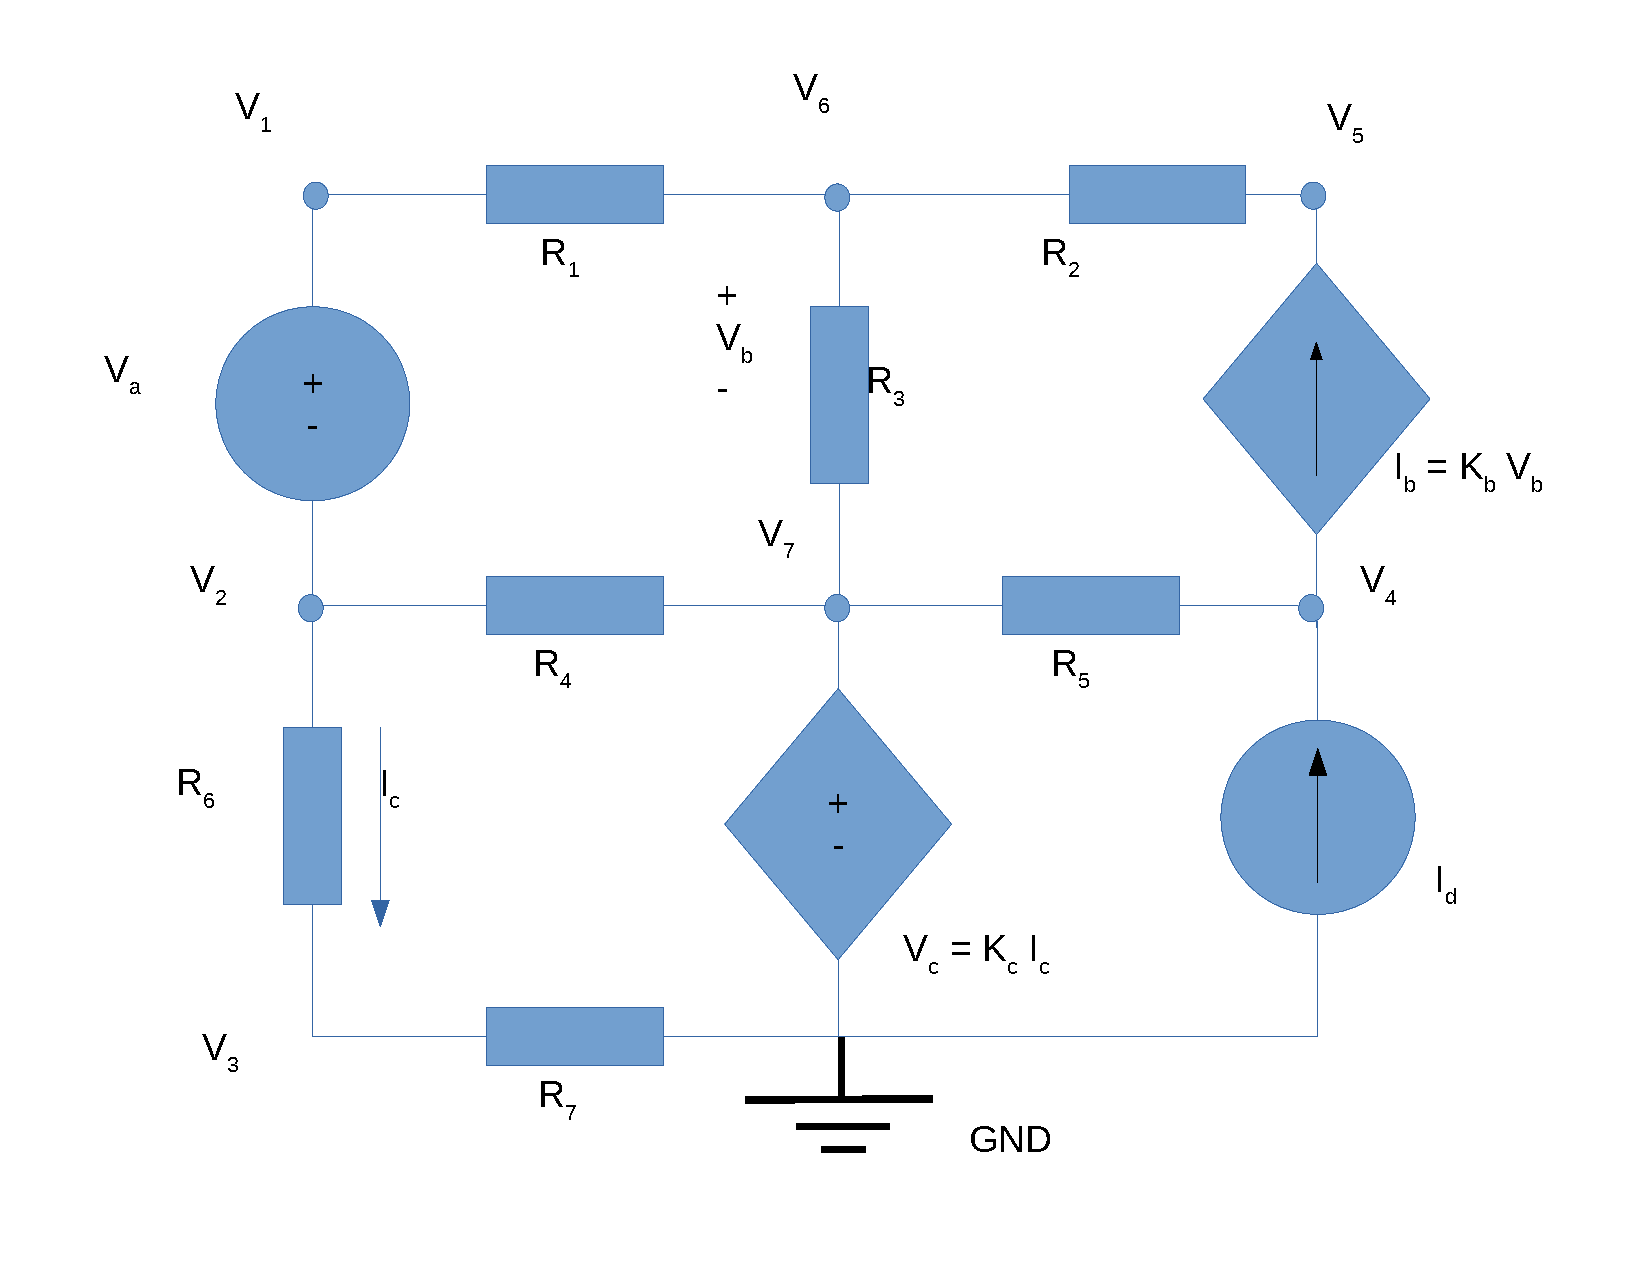
\includegraphics[width=0.8\textwidth, scale=1.0]{rc.pdf}
\squeezeup
\caption{Circuit with an independent current and voltage source ($V_a$ and $I_d$ respectively) and linear dependent sources ($V_c$-linear current controlled voltage source and $I_b$-linear voltage controlled current source}
\label{fig:rc}
\end{figure}

The values given for this report can be found in table~\ref{tab:op1}.

\begin{table}[hb]
  \centering
  \begin{tabular}{|l|r|}
    \hline    
    {\bf Name} & {\bf Values} \\ \hline
    R1 & 1.01949191994 Kohms\\ \hline
R2 & 2.05054429461 Kohms\\ \hline
R3 & 3.09286027724 Kohms\\ \hline
R4 & 4.12838973576 Kohms\\ \hline
R5 & 3.06635427647 Kohms\\ \hline
R6 & 2.01254230153 Kohms\\ \hline
R7 & 1.00502981701 Kohms\\ \hline
Va & 5.24204797361 V\\ \hline
Id & 1.01905568201 mA\\ \hline
Kb & 7.23185131759 mS\\ \hline
Kc & 8.12820254987 Kohms\\ \hline

  \end{tabular}
  \caption{Values received by the Python program.}
  \label{tab:op1}
\end{table}


